\chapter{IIR Lookahead}
\label{chap:iir_lookahead}

In this chapter we will explain how we have improved the original IIR design by applying the techniques studied in the course,
specifically the lookahead first, and later the pipelining and retiming. We derived the new architecture from the block diagram shown in
figure \ref{fig:iir}, then we have modified the C model to obtain a reference implementation and, finally, we have derived
the VHDL implementation to reproduce all the steps done in chapter \ref{chap:iir}. Hence, for this last part, we will
outline only the results and compare them to the IIR's one since the procedures we have followed are the same.

\section{Architecture derivation}

First, as mandated by exercise 2.4, we have applied the J-lookahead method with $J = 1$. This is a non-universal technique,
that is normally applied when other techniques such as pipelining, retiming, unfolding, ecc. cannot be applied. In our baseline
architecture there is actually space for universal techniques, as demonstrated below, although we have applied the lookahead
first nevertheless to comply with the exercise's request.

\subsection{Baseline IIR analysis}

\begin{figure}[!ht]
	\centering
	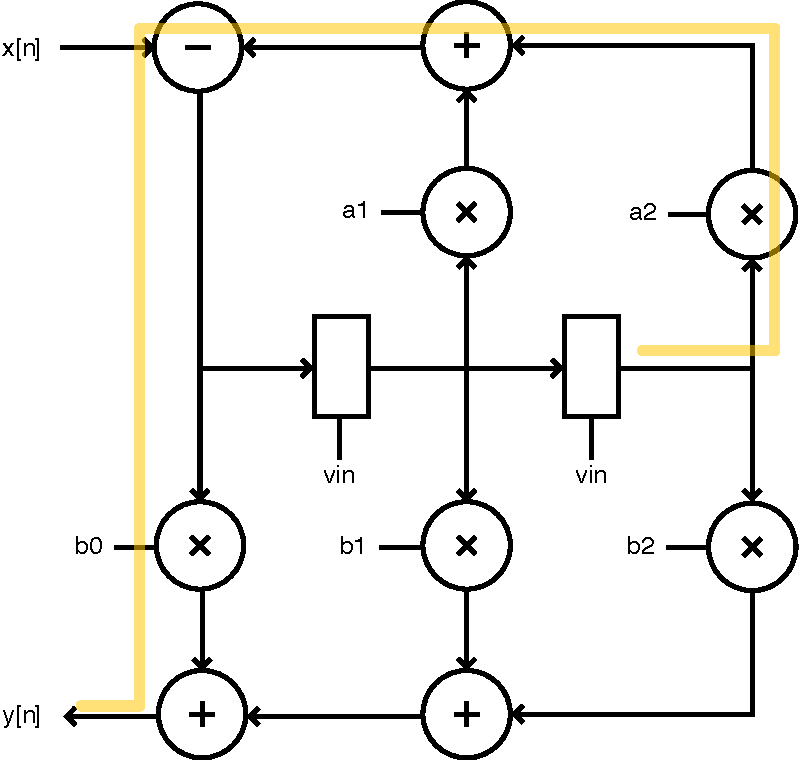
\includegraphics[width=0.4\linewidth]{./chapters/pictures/loop_bound_iir.pdf}
	\caption{Baseline IIR critical path}
	\label{fig:loop_bound_iir}
\end{figure}

In figure \ref{fig:loop_bound_iir} it is outlined in yellow the critical path of the non-optimized filter. If we define with
$T_{a}$ the delay of the adder and with with $T_{m}$ the delay of the multiplier, we obtain that

\begin{equation}
    \label{eq:baseline_iir_delay}
    CP_{iir} = 2T_{m} + 3T_{a}
\end{equation}

It can be also seen in the picture that there are two loops, namely $LB_{1}$ and $LB_{2}$. It is possible to calculate the
loop bound as follows:

\begin{align}\nonumber
    LB_{iir_{1}} = \frac{T_{m} + 2T_{a}}{1} \quad\quad LB_{iir_{2}} = \frac{T_{m} + 2T_{a}}{2}
\end{align}

Hence, we obtain

\begin{equation}\nonumber
    T_{iir_{\infty}} = \max \lbrace LB_{iir_{1}}, LB_{iir_{2}} \rbrace = LB_{iir_{1}} < CP_{iir}
\end{equation}

This means that a universal technique to improve the architecture exists; indeed pipelining could speed-up the architecture,
as there is a feed-forward cut-set which divides the feed-forward multipliers from the upper part of the circuit. By placing
pipeline registers there we would obtain

\begin{equation}
    CP_{iir_{pipeline}} = T_{iir_{\infty}} = T_{m} + 2T_{a}
\end{equation}

This demonstrate that multiple optimization paths do exists for our architecture.

\subsection{Lookahead application}

The lookahead method works by recursively expanding the base equation. As the exercise stated that only one expansion was required,
we have proceeded in this way:

The equation of our filter is

\begin{equation}
    \label{eq:iir_eq}
    \begin{split}
        y[n] &= {\sum_{k=0}^{2} a_{k}y[n-k]} + {\sum_{i=0}^{2} b_{i}x[n-i]} = \\
        &= a_{0}y[n] + a_{1}y[n-1] + a_{2}y[n-2] + b_{0}x[n] + b_{1}x[n-1] + b_2[x-2]
    \end{split}
\end{equation}

We have calculated the formula of $y[n-1]$, which is

\begin{equation}
    \label{eq:yn-1}
    y[n-1] = a_{0}y[n-1] + a_{1}y[n-2] + a_{2}y[n-3] + b_{0}x[n-1] + b_{1}x[n-2] + b_2[x-3]
\end{equation}

If we insert \ref{eq:yn-1} in \ref{eq:iir_eq} the result is

\begin{equation}
    \label{eq:lookahead}
    \begin{split}
        y[n] &= a_{0}y[n] + a_{1}a_{0}y[n-1] + a^2_{1}y[n-2] + a_{1}a_{2}y[n-3] + a_{1}b_{0}x[n-1] + a_{1}b_{1}x[n-2]\ + \\
    & + a_{1}b_{2}x[n-3] + a_{2}y[n-2] + b_{0}x[n] + b_{1}x[n-1] + b_{2}x[n-2]
    \end{split}
\end{equation}

Which is our new filter's equation. Its block diagram is shown in figure \ref{fig:iir_lookahead}.

\begin{figure}[!ht]
	\centering
	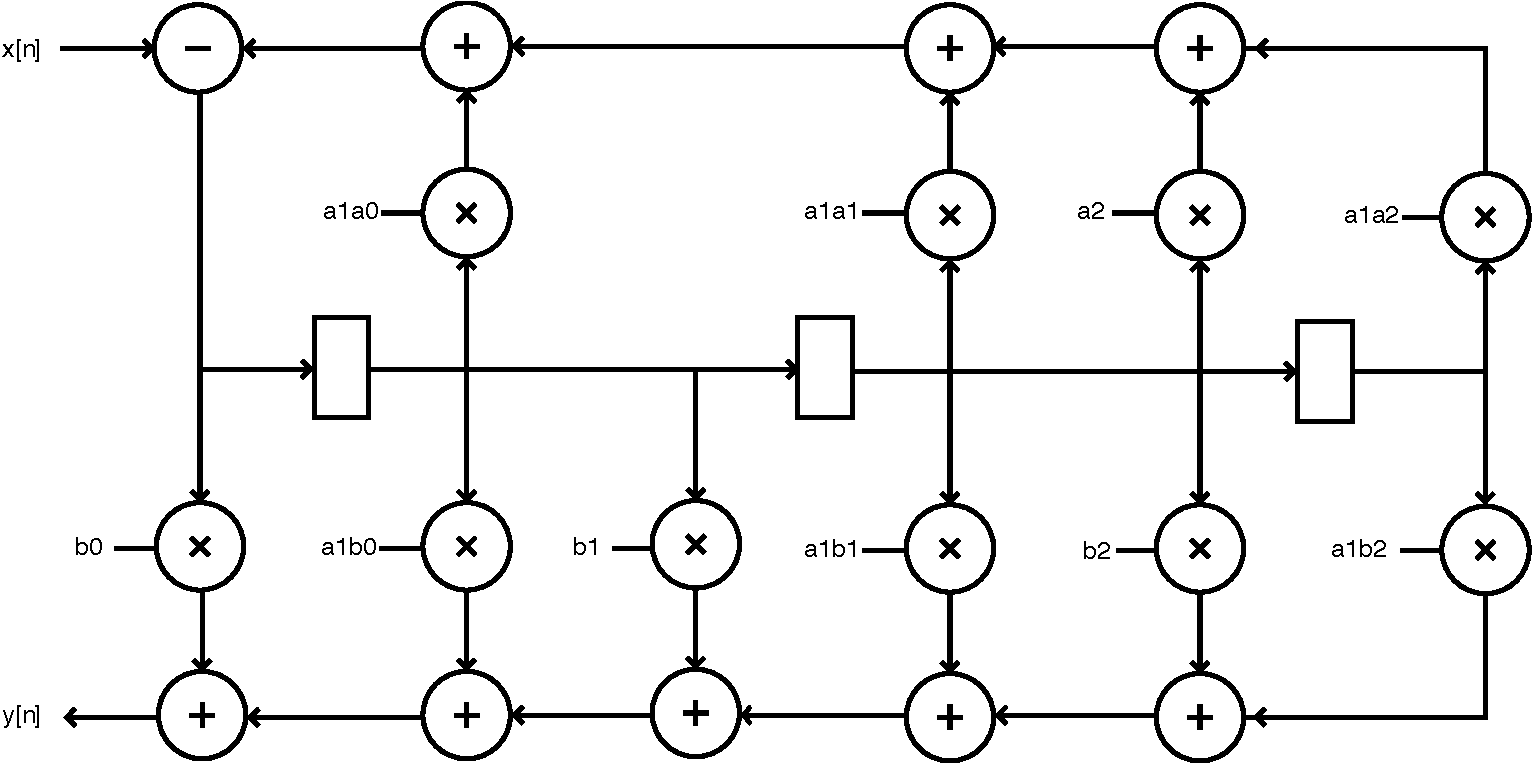
\includegraphics[width=0.7\linewidth]{./chapters/pictures/iir_lookahead.pdf}
	\caption{IIR lookahead}
	\label{fig:iir_lookahead}
\end{figure}

In equation \ref{eq:lookahead} it can be noticed that new coefficients appear in the form $a_{1}*a_{j}$ and $a_{1}*b_{j}$.
Their result does not fit in 12 bits, therefore we have decided to truncate them (by taking the 12 MSBs) to respect the original interface's bit width.

Starting from the structure shown in figure \ref{fig:iir_lookahead} we have derived a new C and VHDL model: the latter has been used as basis for the
optimizations described in section \ref{sec:iir_opt}, the former as golden model to check the results since, due to the new coefficients, the filter
has a different $THD$ and produces slightly different values. 

\section{Lookahead optimizations}
\label{sec:iir_opt}

Before applying any universal optimization technique, as always we needed to check if

$$T_{lookahead_{\infty}} < CP_{lookahead}$$

\begin{figure}[!ht]
	\centering
	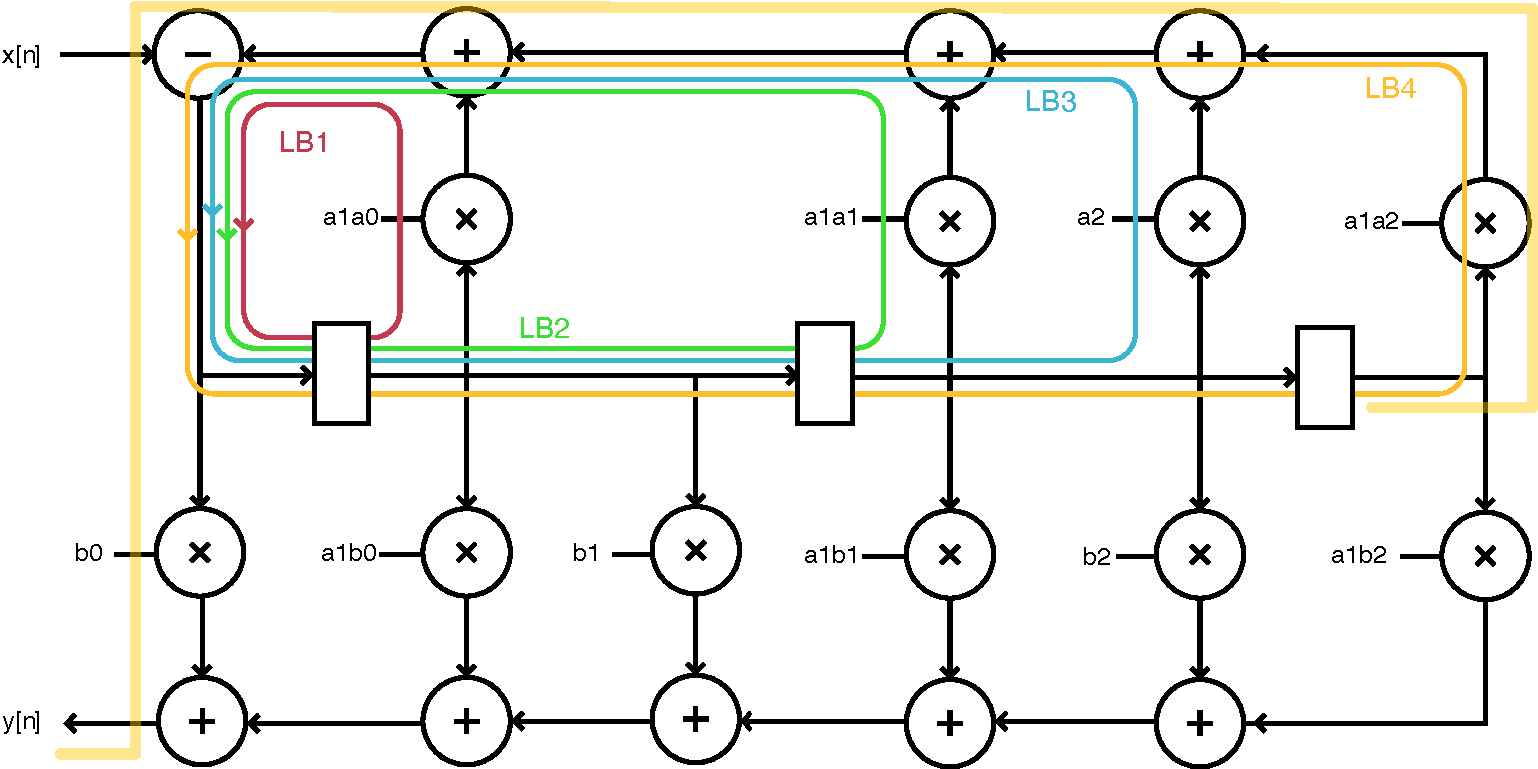
\includegraphics[width=0.7\linewidth]{./chapters/pictures/loop_bound_iir_lookahead.pdf}
	\caption{IIR lookahead critical path and loop bounds}
	\label{fig:lookahead_lb}
\end{figure}

In yellow it is highlighted the new critical path, which is equal to

\begin{equation}\nonumber
    \label{eq:lookahead_cp}
    CP_{lookahead} = 2T_{m} + 5T_{a}
\end{equation}

While in red, green, blue and orange are highlighted all the design's loops, which are respectively $LB_{1}$, $LB_{2}$, $LB_{3}$, $LB_{4}$ and are equal to

\begin{align}\nonumber
    &LB_{lookahead_{1}} = \frac{T_{m} + 2T_{a}}{1} &LB_{lookahead_{2}} = \frac{T_{m} + 3T_{a}}{2} \\ \nonumber
    &LB_{lookahead_{3}} = \frac{T_{m} + 4T_{a}}{2} &LB_{lookahead_{4}} = \frac{T_{m} + 4T_{a}}{3} \nonumber
\end{align}

Again, we have calculated $T_{lookahead_{\infty}}$ as

\begin{equation}\nonumber
    T_{lookahead_{\infty}} = \max \lbrace LB_{lookahead_{1}}, LB_{lookahead_{2}}, LB_{lookahead_{3}}, LB_{lookahead_{4}} \rbrace = LB_{lookahead_{1}}
\end{equation}

Which is smaller than $CP_{lookahead}$. To have $T_{lookahead_{\infty}} = CP_{lookahead}$ we have applied a combination of retiming and pipelining, as
shown in figure \ref{fig:lookahead_opt}.

\begin{figure}[!ht]
	\centering
	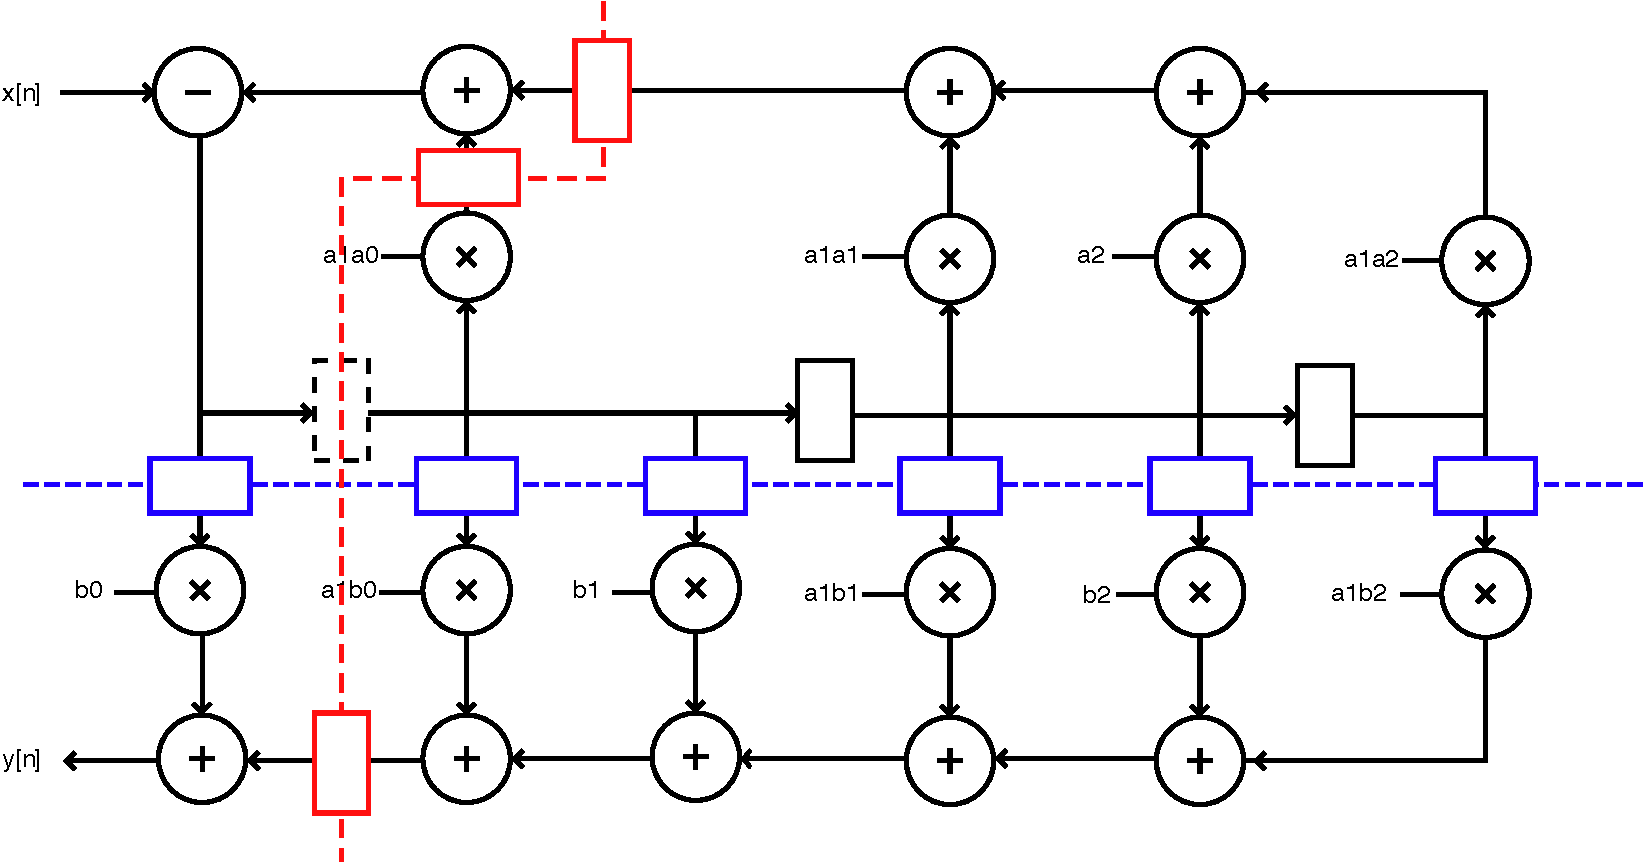
\includegraphics[width=0.8\linewidth]{./chapters/pictures/iir_opt.pdf}
	\caption{Optimized IIR lookahead}
	\label{fig:lookahead_opt}
\end{figure}

First, we applied retiming on the leftmost register, which is the dashed black one, by using the cut-set shown in red. With the same color are shown the
retiming registers. Furthermore, in blue it is shown the forward cut-set used for pipelining and the related registers.
Pipelining, in respect to retiming, changes the behavior of the circuit. Indeed it had consequences on the delay of the $vin$ signal, which has been
adjusted accordingly. The new critical path has now a delay of

\begin{equation}
    \label{eq:lookahead_opt_delay}
    CP_{lookahead} = T_{m} + 2T_{a}
\end{equation}

Which is better than the one of the baseline IIR described in equation \ref{eq:baseline_iir_delay}.

\subsection{Logic synthesis results}

We have updated the script described in the previous chapter to synthesize this architecture.
The smallest $t_{ck}$ we have been able to achieve is $t_{ck_{min}} = 2.55\ ns$, with a corresponding
area of $A_{min} \approx 8605\ \mu m^2$.

By using $t_{ck} = 4*t_{ck_{min}} = 10.6\ ns$ the design is able to provide a value after $3.43\ ns$ with a slack of $7.06\ ns$.
The area, in this case, is equal to $A \approx 7958\ \mu m^2$.

As already done in the previous chapter, we can see that for a speed reduction of $\approx 34.5\%$ there is an area gain of $\approx 7.5\%$.

\subsection{Power consumption estimation}

After the synthesis we have run a simulation to verify the correctness of the synthesized file and its switching activity as explained in the previous
chapter. The power report is listed below.

\begin{Verbatim}[fontsize=\footnotesize]
Cell Internal Power  = 689.3951 uW   (57%)
Net Switching Power  = 515.5695 uW   (43%)
                        ---------
Total Dynamic Power    =   1.2050 mW  (100%)

Cell Leakage Power     = 163.5452 uW


                Internal         Switching           Leakage            Total
Power Group      Power            Power               Power              Power   (   %    )  Attrs
--------------------------------------------------------------------------------------------------
io_pad             0.0000            0.0000            0.0000            0.0000  (   0.00%)
memory             0.0000            0.0000            0.0000            0.0000  (   0.00%)
black_box          0.0000            0.0000            0.0000            0.0000  (   0.00%)
clock_network      0.0000            0.0000            0.0000            0.0000  (   0.00%)
register         219.9684           71.4661        2.5763e+04          317.1974  (  23.18%)
sequential         0.0000            0.0000            0.0000            0.0000  (   0.00%)
combinational    469.4267          444.1043        1.3778e+05        1.0513e+03  (  76.82%)
--------------------------------------------------------------------------------------------------
Total            689.3951 uW       515.5704 uW     1.6355e+05 nW     1.3685e+03 uW
\end{Verbatim}

\subsection{Place and route results}

Again, we have repeated the same steps of the baseline IIR and we report here for commodity the power consumption report after the place \& route.

\begin{Verbatim}[fontsize=\footnotesize]
Total Power [Power Units = 1mW]
-----------------------------------------------------------------------------------------
Total Internal Power:        1.73352686 	   54.5286%
Total Switching Power:       1.28357305 	   40.3752%
Total Leakage Power:         0.16201317 	    5.0962%
Total Power:                 3.17911308 
-----------------------------------------------------------------------------------------


Group                           Internal   Switching     Leakage       Total  Percentage 
                                Power      Power         Power         Power  (%)        
-----------------------------------------------------------------------------------------
Sequential                        0.2444     0.07291     0.02576      0.3431       10.79 
Macro                                  0           0           0           0           0 
IO                                     0           0           0           0           0 
Combinational                      1.489       1.211      0.1363       2.836       89.21 
Clock (Combinational)                  0           0           0           0           0 
Clock (Sequential)                     0           0           0           0           0 
-----------------------------------------------------------------------------------------
Total                              1.734       1.284       0.162       3.179         100 
-----------------------------------------------------------------------------------------
    
    \end{Verbatim}

\section{Final results analysis}

The lookahead version of the IIR is faster and more area and power hungry in respect to the baseline IIR.
In table \ref{tab:comparison} the improvement in percentage of the lookahead with respect to the baseline filter
is summarized. A negative percentage indicates a worsening, eg. if the area is negative then the lookahead
is larger than the baseline.

\begin{center}
    \label{tab:comparison}
    \begin{tabular}{ |c|c|c| }
        \hline
        Metric & $t_{ck_{min}}$ & $4t_{ck_{min}}$ \\
        \hline
        Timing & $9\%$ & $33\%$ \\
        \hline
        Area & $-102\%$ & $-115\%$ \\
        \hline
        Power & - & $-125\%$ \\
        \hline
    \end{tabular}
\end{center}

Given these numbers it is clear that the IIR lookahead should be used only when speed is of paramount importance, since the worsening normally
outweigh the speed benefit.

Moreover, even when talking about speed, the percentage difference between the two $t_{ck_{min}}$ is marginal, as it is only $9\%$ even if
$CP_{iir} > CP_{lookahead}$ (eq. \ref{eq:baseline_iir_delay}, \ref{eq:lookahead_opt_delay}). We suppose that this is due to the ability of the
synthesizer to find more optimization opportunities thanks to the longer combinational path, probably by merging adders and/or multipliers together.
The improvements given by pipelining and retiming are noticeable only when using $t_{ck} = 4t_{ck_{min}}$ since the lookahead architecture is $33\%$ faster
than the baseline one.

We think, however, that this result could be reverted by pipelining the baseline IIR, since it would reach the same $CP$ length with less hardware.